\documentclass{article}
\usepackage{listings}
\usepackage{xcolor}
\usepackage{graphicx}
\definecolor{codegreen}{rgb}{0,0.6,0}
\definecolor{codegray}{rgb}{0.5,0.5,0.5}
\definecolor{codepurple}{rgb}{0.58,0,0.82}
\definecolor{backcolour}{rgb}{0.95,0.95,0.92}

\lstdefinestyle{mystyle}{
    backgroundcolor=\color{backcolour},   
    commentstyle=\color{codegreen},
    keywordstyle=\color{magenta},
    numberstyle=\tiny\color{codegray},
    stringstyle=\color{codepurple},
    basicstyle=\ttfamily\footnotesize,
    breakatwhitespace=false,         
    breaklines=true,                 
    captionpos=b,                    
    keepspaces=true,                 
    numbers=left,                    
    numbersep=5pt,                  
    showspaces=false,                
    showstringspaces=false,
    showtabs=false,                  
    tabsize=2
}

\lstset{style=mystyle}

\begin{document}

\section{SQL: Language characteristics}

SQL is short for \textbf{Structured Query Language}
\begin{itemize}
    \item Language to operate databases and provides an interface with RDBMS (\textbf{Relation Database Management System})
    \begin{itemize}
        \item Database creation
        \item Data loading
        \item Data modification
    \end{itemize}
    \item SQL has 3 different types of instructions 
    \begin{enumerate}
        \item Data Control Language 
        \begin{itemize}
            \item Grant, Revoke
            \item Is concerned with acces privilige and determines who can control which part of the database 
        \end{itemize}
        \item Data Manipulation Language 
        \begin{itemize}
            \item Select, insert, update, delete
            \item Data retrieval, removal and transformation
        \end{itemize}
        \item Data Definition Language
        \begin{itemize}
            \item Create, drop, alter
            \item Creation and maintenance of databases, tables, views, indices
        \end{itemize}
    \end{enumerate}
    \item SQL is based on the relational model of data
    \begin{itemize}
        \item Tables, 2D datastructes consisting of rows and columns 
        \item Rows (instance/record) is a collection of different characteristics that all belong to the same datapoint
        \item Column (attribute) is a collection of data describing one specific characteristic over different instances
        \item Field is the intersection between a column and a row 
        \item Primary key, a unique identifier that defines an instance 
        \item Foreign key, a connecting key between two different tables
    \end{itemize}
\end{itemize}

\section{Selecting data}

\subsection{SELECT command}

The \textbf{SELECT} statement allows us to specifiy which data we wish to call from the database in order to view, manipulate, etc.
The general synthax for the SELECT statement can be written as 

\begin{lstlisting}[frame=single]
    SELECT [Predicate] {* | table.* | [table.]field1 [, [table.]field2 [,...]]} FROM tableexpression
\end{lstlisting}

The SELECT statement consists of different components
\begin{itemize}
    \item \textbf{Predicate}, a signifier that lets us control which records are displayed
    \begin{itemize}
        \item \textbf{ALL} takes all the data that is present in the ranges we specify
        \item \textbf{DISTINCT} returns only an overview of the possible values in the 
    \end{itemize}
    \item Field or table specifiers where we can control which tables or which section of a table we wish to select 
    \begin{itemize}
        \item \textbf{*}, denotes to select everything 
        \item \textbf{tableName}
        \item \textbf{tableName.fieldName}
        \item multiple tables and/or fields can be selected at once using a \textbf{,} as a seperation
    \end{itemize} 
    \item \textbf{FROM} denotes where our selection comes from 
    \begin{itemize}
        \item table
        \item tableexpression, linking multiple tables to each other
    \end{itemize} 
\end{itemize}

\subsection{WHERE command}

The \textbf{WHERE} works as a filter that allows us to retrieve data that needs to fulfill a specific condition or multiple conditions
\begin{lstlisting}[frame=single]
    WHERE attribute operator constant | attribuut 
\end{lstlisting}

The WHERE statement consists of different components
\begin{enumerate}
    \item \textbf{Attribute} determines which column we will be filtering
    \item \textbf{Operator} specifies the condition that needs to be fulfilled
    \begin{itemize}
        \item =, equality operator 
        \item \(<,>, <=, >=\), greater/lesser than
        \item \(<>, !=\), not equal operator 
        \item BETWEEN, the range operator
        \item LIKE, pattern operator using the wildcard operators '\%' and '\_'
        \begin{itemize}
            \item '\%', represents multiple characters (or nothing) that can be anything
            \begin{itemize}
                \item 'c\%' with c as any character searches for anything starting with the character c
                \item '\%c\%' with c as any character searches for anything that contains the character in the entry
                \item '\%c' with c as any character searches for anything that ends with the character c
            \end{itemize}
            \item '\_' represents a single character (or nothing) that can be anything
            \begin{itemize}
                \item 'c\_' with c as any character searches for anything starting with the character c followed by one other character due to the single underscore
                \item '\_c\_' with c as any character searches for anything that contains the character c between two characters due to the single underscore before and after the letter
                \item '\_c' with c as any character searches for anything that ends with the character c following a single character
                \item A repetition of multiple underscores looks for anything that has the same length as the number of underscores 
            \end{itemize} 
        \end{itemize}
    \end{itemize}
\end{enumerate}
The WHERE statement can be combined with logical operators 
\begin{itemize}
    \item AND, requires both conditions to be fulfilled 
    \item OR, requires one of the conditions to be fulfilled 
    \item NOT, requires the condition not to be fulfilled
\end{itemize}

\subsection{ORDER BY command}

ORDER BY command imposes an ordering upon the data retrieved by the query. When using ORDER BY the collation, i.e. differentiation between smaller and capital letters, is dependant on the setting.
As a standard mysql does not differentiate between capital letters and lowercase letters.
\begin{lstlisting}[frame=single]
    ORDER BY attribuut asc|desc
\end{lstlisting}
\begin{itemize}
    \item Ordering always happens based on the values of an attribute 
    \item asc orders the values from smallest to largest (ascending). When the values are strings the ordering happens from A to Z
    \item desc orders the values from largest to smallest (descending). When the values are strings the ordering happens from Z to A
\end{itemize}
Sorting on mulitple attributes is possible, it should be noted that sorting happens in a sequential fashion. Changing the order changes the output of the query.

\subsection{AGGREGATE functions}

AGGREGATE functions performs specific computations on a given variable where all recors that are non NULL are taken into account
\begin{itemize}
    \item COUNT, gives a frequency distribution of each value 
    \item SUM, sums up all the entries
    \item AVG, averages out over all the entries
    \item MAX/MIN, finds the upper and lower value in the parameter
\end{itemize}

\begin{lstlisting}[frame=single]
    AGGREGATE(paramName) [as ALIAS]
\end{lstlisting}
\begin{itemize}
    \item Similar syntax as functions in programming language where the AGGREGATE is one of the functions mentioned above
    \item [as ALIAS], optional syntax that allows us to rename the AGGREGATE to an alias of choice 
\end{itemize}

\subsection{GROUP BY command}

GROUP BY is used to cluster rows that fulfill a specific condition together which allows us to perform AGGREGATE functions on subsets of the data instead of the data in its entirety.
A commonly used keyword in the GROUP BY command is the HAVING keyword. The HAVING keyword functions as a filter but is not equivalent to the WHERE keyword 
\begin{itemize}
    \item WHERE
    \begin{itemize}
        \item  used to filter the records from the table based on the specified condition.
        \item can be used without GROUP BY Clause
        \item implements in row operations
        \item cannot contain aggregate function
        \item can be used with SELECT, UPDATE, DELETE statement
        \item is used before GROUP BY Clause
        \item is used with single row function like UPPER, LOWER etc.
    \end{itemize} 
    \item HAVING
    \begin{itemize}
        \item is used to filter record from the groups based on the specified condition
        \item cannot be used without GROUP BY Clause
        \item implements in column operation
        \item can contain aggregate function
        \item can only be used with SELECT statement
    \end{itemize}
\end{itemize}

\begin{lstlisting}[frame=single]
    SELECT [AGGREGATE]colName(s) FROM tableName WHERE condition(s) GROUP BY colName(s) HAVING condition(s) ORDER BY ASC | DESC
\end{lstlisting}
\begin{itemize}
    \item GROUP BY should always be placed in front of ORDER BY
    \item If ORDER BY is not used the result will be sorted based on the columns of GROUP BY
    \item When using the GROUP BY statement then we need to include all columns that are not aggregated to be mentioned in the GROUP BY clause
\end{itemize}

\section{Working with mulitple tables}

\subsection{Inner join}

An inner join is a way of combining multiple tables together where the tables display overlap between their data. 
The inner join can be visualized with the following diagram
\begin{center}
    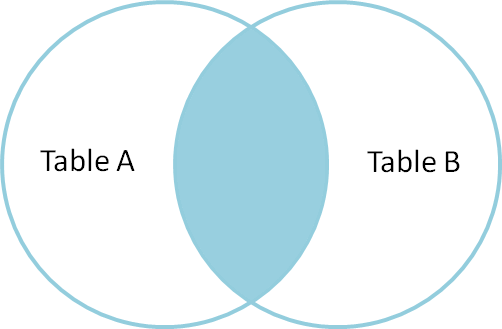
\includegraphics[scale=0.5]{img/innerjoin.png}
\end{center}
Only those rows/records that are matching in both the tables will be included the formation of a merged table.
The inner join is used by the command 
\begin{lstlisting}[frame=single]
    select cols from table_1 inner join table_2 on col_condition(t1_col operator t2_col) [inner join table_3 on col_condition]
\end{lstlisting}
\begin{itemize}
    \item The condition on which we decide which data is to be included is determined by a comparison between the data of both table. Valid operators are '=', '$<$', '$>$', '$<=$', '$>=$', '$!=$ or $<>$'
    \item Multiple conditions can be formulated for the inner join using the AND or OR keywords
    \item Mulitple tables can be joined simultaneously by following an inner join with another. This results in a new table in which we look for data that is overlapping between multiple tables
    \begin{center}
        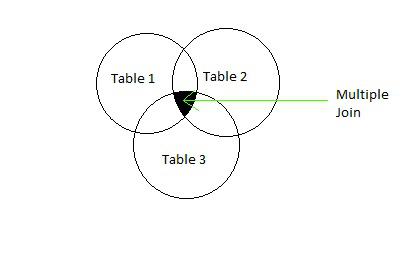
\includegraphics{img/multipleInner.jpg}
    \end{center}
\end{itemize}

\subsection{Outer join}

Outer join allows us to combine 2 tables together based on a specific condition similarly to how the inner join was used.
The major difference between the inner and outer join operations is that outer join allows us to include non overlapping data into the end result of our query.
The outer join can be differentiated using the keywords left and right
\begin{itemize}
    \item left outer join takes the non overlapping data from the first table 
    \item right outer join takes the non overlapping data from the second table 
\end{itemize}
The outer join operation can be represented through the following diagram
\begin{figure}
    \centering
    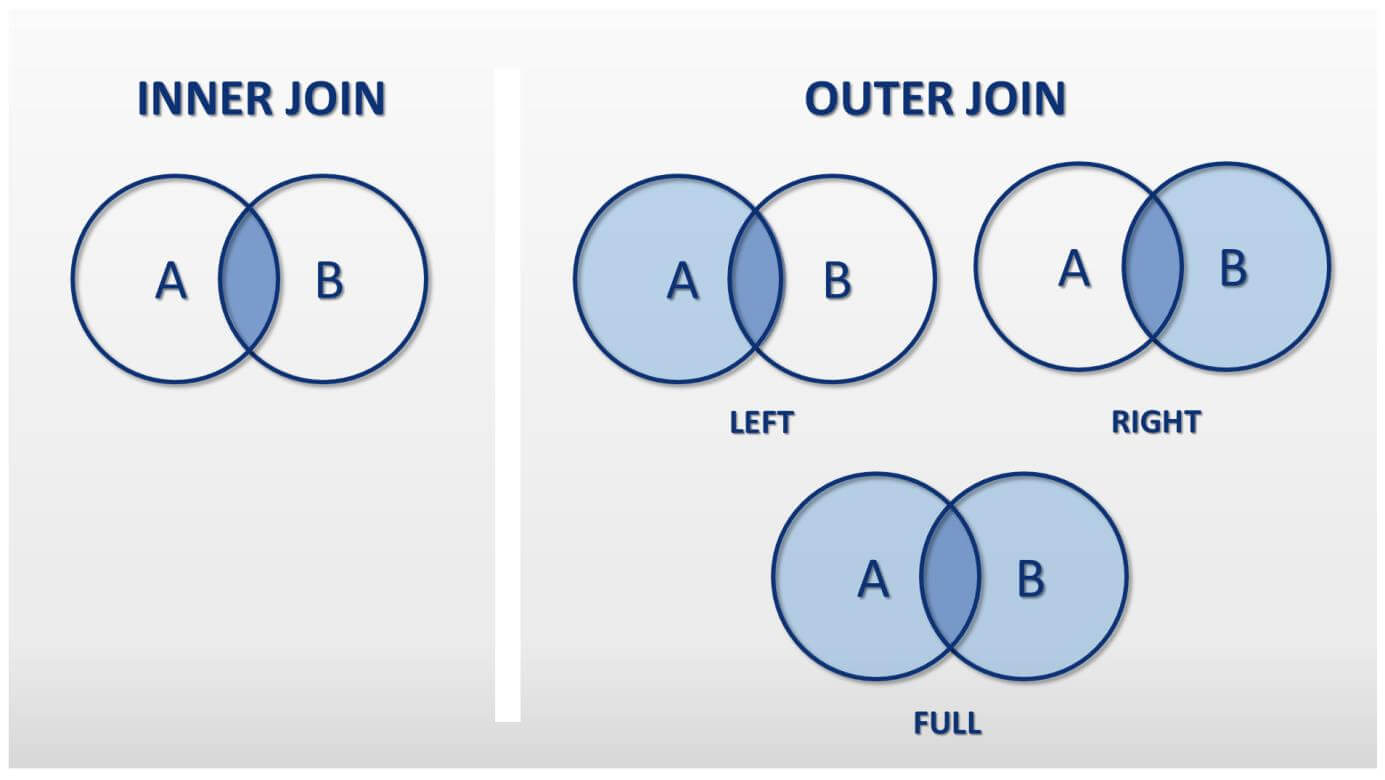
\includegraphics[width=\linewidth]{img/Outer-Join.jpg}
    \caption{Different outer join operations contrasted against the inner join. Outer join adds upon the inner join by taking the data that is not present in the overlap between tables}
\end{figure}

\begin{lstlisting}[frame=single]
    select cols from table_1 [left | right] (outer) join table_2 on col_condition
\end{lstlisting}
\begin{itemize}
    \item Outer is an optional keyword in this case and does not need to be included into the query
\end{itemize}

Outer joins and inner joins can be combined together by nesting the joining operations. However \textbf{an outer join can not be followed by an inner join}. Despite the fact that this is possible to do in SQL and it will not result in a query error, the result that is generated will be faulty.
This is due to the nature of the joining operations that are used.
\begin{itemize}
    \item Outer join specifically includes \textbf{non overlapping data} in the query result where as the inner join will \textbf{only return that information which is overlapping between tables}
    \item Using an inner join \textbf{after} an outer join will \textbf{negate the whole point of the outer join}
\end{itemize}

\subsection{Self join}

The self join allows us to combine a table with it self 

\begin{lstlisting}[frame=single]
    select cols from table as t1 join table as t2 on t1.col operator t2.col
\end{lstlisting}
\begin{itemize}
    \item The table has to have a 2 references in order for this to work
\end{itemize}

\section{Mulitple queries}

\subsection{Union}

Multiple queries can be combined into a single result by using the union statement 

\begin{lstlisting}[frame=single]
    query_1 union query_2 ... union query_n
    query_i: select ...
\end{lstlisting}
\begin{itemize}
    \item Each query in the union needs to select the \textbf{same amount fields or columns}. The fields do \textbf{not need to have the same amount of records or rows}
    \item Only the first query can be given an alias 
    \item order by can be used but needs to be included at the end of the union. 
    \item If the same fields are in mulitple queries then they will only be returned once. You can force the display of duplicate results using the union all command.
\end{itemize}

\subsection{Subqueries}

It is possible to incorperate queries into another query, i.e. multiple selects into a single query 
\begin{itemize}
    \item where select \dots
    \item having select \dots
    \item select select \dots
    \item from select \dots
    \item Insert, update, delete 
\end{itemize}
A special kind of subquery is the \textbf{correlated subquery}. This subquery is a query where we refer to a table that appears \textbf{in the outer query}.
An example of a correlated subquery is 
\begin{lstlisting}[frame=single]
    select * from t1 where c1 any (select c1 from t2 where t2.c2=t1.c2)
\end{lstlisting}
It is important to remember that SQL \textbf{evaluates from inside to outside}

\section{Modifying tables and data}

\subsection{INSERT command}

The insert command allows us to append a new row to an existing table.
The command is build up with the following syntax 
\begin{lstlisting}[frame=single]
    insert into tablename [(col1name, col2name, \dots)] values (col1val, col2val, \dots)
\end{lstlisting}
\begin{itemize}
    \item The target columns is not required when using the insert statement but it is advised. When not including the the names of the columns the insert function will take the order of the columns as it is stored. If we give an ordering of the columns in the statement then the values will be appended in the same order as our column order
    \item Column names are placed between round brackets after the table name
    \item Depending on the data type we use a different formating
    \begin{itemize}
        \item Quotation marks are used for non numerical data 
        \item Different values are seperated with a comma
    \end{itemize}
    \item Mulitple values can be appended at once. These are added by seperating each row of values with round brackets 
    \begin{lstlisting}[frame=single]
        insert into tablename [(col1name, col2name, \dots)] values (col1val, col2val, \dots), (col1val, col2val, \dots), \dots        
    \end{lstlisting}
\end{itemize}
Values from other tables can be appended to an existing table with the insert statement. When extracting data from a different table we use a select query for the colvalues
\begin{lstlisting}[frame=single]
    insert into tablename1 [(col1name, col2name, \dots)] select tablename2.colname from tableexpression where \dots 
\end{lstlisting}

\end{document}